% SCoPe final report, IEEE conference format (IEEEtran).
% Build: run report/make_assets.py and report/make_bib.js, then pdflatex main.tex twice.
% Every number below comes from generated/numbers.tex and the generated tables, which are
% produced from the run logs; nothing measured is typed by hand except where a sentence says so.
\documentclass[conference]{IEEEtran}
\IEEEoverridecommandlockouts
\usepackage{cite}
\usepackage{amsmath,amssymb,amsfonts}
\usepackage{graphicx}
\usepackage{booktabs}
\usepackage{multirow}
\usepackage{xcolor}
\usepackage{algorithm}
\usepackage{algpseudocode}
\usepackage{balance}
\usepackage[hidelinks]{hyperref}
\usepackage{url}
\def\UrlBreaks{\do\/\do-\do.}

% generated by report/make_assets.py; do not edit
\newcommand{\PushTSeeds}{3}
\newcommand{\PushTRoneMean}{0.873}
\newcommand{\PushTRoneSD}{0.046}
\newcommand{\PushTFinalMean}{0.900}
\newcommand{\PushTFinalSD}{0.053}
\newcommand{\PushTFinalRound}{3}
\newcommand{\PushTPerSeedFinal}{0.92 / 0.94 / 0.84}
\newcommand{\WallSeeds}{3}
\newcommand{\WallRoneMean}{0.520}
\newcommand{\WallRoneSD}{0.020}
\newcommand{\WallFinalMean}{0.947}
\newcommand{\WallFinalSD}{0.023}
\newcommand{\WallFinalRound}{3}
\newcommand{\WallPerSeedFinal}{0.92 / 0.96 / 0.96}
\newcommand{\MazeSeeds}{1}
\newcommand{\MazeRoneMean}{0.860}
\newcommand{\MazeRoneSD}{--}
\newcommand{\MazeFinalMean}{1.000}
\newcommand{\MazeFinalSD}{--}
\newcommand{\MazeFinalRound}{2}
\newcommand{\MazePerSeedFinal}{1.00}
\newcommand{\HSeeds}{3}
\newcommand{\HSeedWord}{3 seeds}
\newcommand{\HEpisodes}{80}
\newcommand{\HPairs}{76{,}800}
\newcommand{\HBest}{MC-dropout}
\newcommand{\HMC}{0.86}
\newcommand{\HMCCI}{0.84--0.88}
\newcommand{\HDist}{0.79}
\newcommand{\HDistCI}{0.76--0.82}
\newcommand{\HRand}{0.50}
\newcommand{\HRandCI}{0.49--0.51}
\newcommand{\HAct}{0.66}
\newcommand{\HActCI}{0.64--0.67}
\newcommand{\HKnn}{0.62}
\newcommand{\HKnnCI}{0.56--0.66}
\newcommand{\HObs}{0.50}
\newcommand{\HObsCI}{0.44--0.55}
\newcommand{\HCost}{0.51}
\newcommand{\HCostCI}{0.47--0.55}
\newcommand{\HCombo}{0.85}
\newcommand{\HComboCI}{0.83--0.87}
\newcommand{\HMCPerSeed}{0.87, 0.84, 0.88}
\newcommand{\HMCSeedMin}{0.84}
\newcommand{\HMCSeedMax}{0.88}
\newcommand{\GatePlain}{71.3\%}
\newcommand{\GateOracle}{72.5\%}
\newcommand{\GateRandom}{70\%}
\newcommand{\GateMC}{70\%}
\newcommand{\GateStep}{1.3\%}

\newcommand{\Rset}{\mathbb{R}}

\begin{document}

\title{SCoPe: Trust-Region Latent Planning\\with JEPA World Models}

\author{\IEEEauthorblockN{[TEAM MEMBER 1], [TEAM MEMBER 2]}
\IEEEauthorblockA{\textit{[Department]}, \textit{[Institution]}\\
Guide: [GUIDE NAME]\\
\{[email]\}}}

\maketitle

\begin{abstract}
Planners built on learned world models choose the action sequence whose \emph{imagined} outcome looks best, but they
trust every imagined future equally, including the ones the model gets badly wrong. We study SCoPe, a decision-time
check for latent model-predictive control (MPC) with a frozen joint-embedding predictive (JEPA) world model: every
imagined step of every candidate plan receives a trust score, and candidates that leave the region where the model is
reliable are rejected before a plan is chosen. Building on DINO-WM, we first reproduce its planning results on an
8\,GB laptop GPU, made feasible by runtime patches that cut rollout time 3.8$\times$ without changing any decision of the
cross-entropy-method (CEM) planner: Push-T reaches \PushTFinalMean{} over \PushTSeeds{} seeds (published 0.90), Wall
\WallFinalMean{} over \WallSeeds{} seeds (0.96) and PointMaze \MazeFinalMean{} (0.98). We then test the first hypothesis of
SCoPe offline: on \HPairs{} imagined steps checked against the simulator, an untrained Monte-Carlo-dropout score
identifies the steps with the largest real latent error at AUROC \HMC{} (95\% CI \HMCCI{}), above both a random score
(\HRand{}) and a strong trivial control (\HDist{}). An offline replay of the gate on recorded candidates, however, barely
changes plan success, even with an oracle gate, so the benefit of gating has to be established in closed loop. We
report both findings, the protocol, and the remaining steps.
\end{abstract}

\begin{IEEEkeywords}
world models, model-based reinforcement learning, model-predictive control, JEPA, uncertainty estimation
\end{IEEEkeywords}

% ======================================================================
\section{Introduction}

A robot can plan by imagining the consequences of its actions with a learned world model and executing the action
sequence whose imagined result is closest to its goal. Joint-embedding predictive architectures (JEPA)~\cite{ref5,ref4}
make this practical from images: instead of predicting pixels, they predict the future in the embedding space of a
pretrained encoder. DINO-WM~\cite{ref1} combines a frozen DINOv2 encoder~\cite{ref3} with a learned latent predictor and
plans with the cross-entropy method (CEM) inside MPC, reaching 90\% success on the Push-T manipulation task without any
reward or task-specific training; V-JEPA~2-AC~\cite{ref2} applies the same idea to real robot arms.

These planners have a blind spot: the planner selects the candidate whose imagined future scores best and never asks
whether that imagination is reliable. Fig.~\ref{fig:failure} shows a case from our own runs: the model imagines the
T-shaped block rotating onto the goal, the planner commits to the plan, and in the simulator the block barely moves.
Prediction errors also grow with the horizon, and simply penalising uncertainty can backfire~\cite{ref18}.

\begin{figure*}[t]
\centering
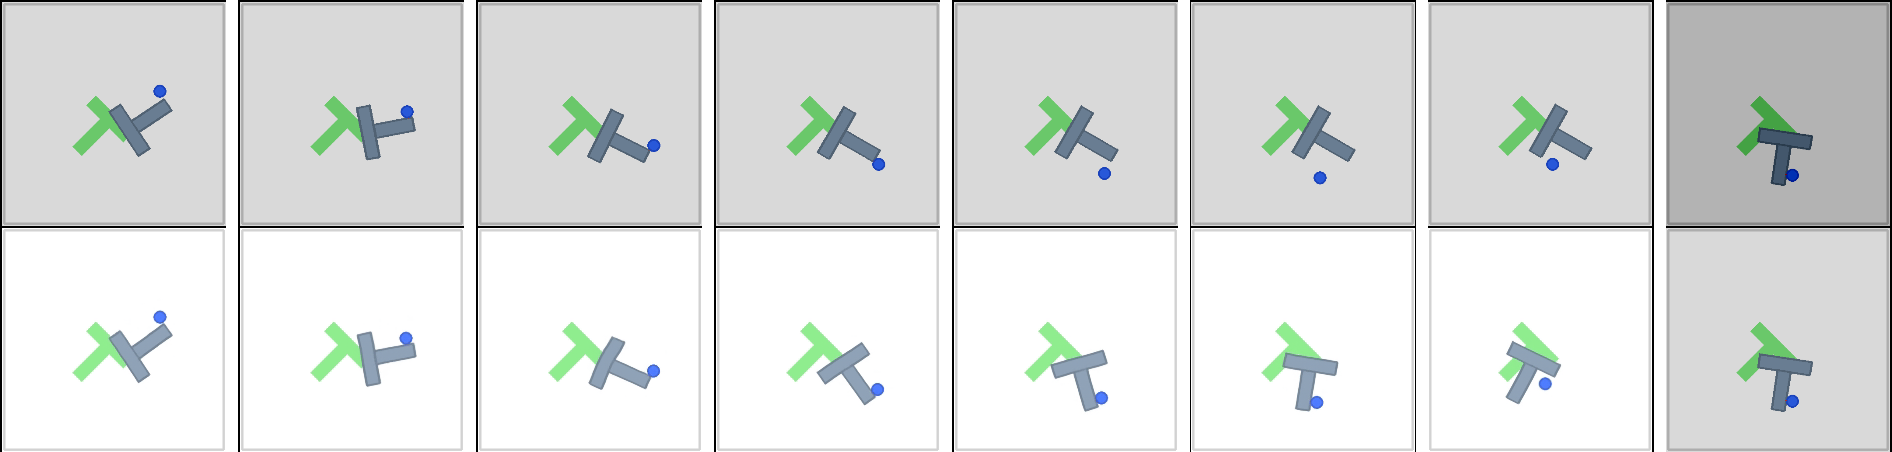
\includegraphics[width=0.86\textwidth]{figures/fig_failure.png}
\caption{A logged failure (Push-T, seed 101, episode 0, simulator steps 0--25 and the goal). Top: what happened in the
simulator. Bottom: what DINO-WM imagined for the same actions. The imagined block reaches the goal pose; the real one
barely moves, and the episode is never solved. SCoPe aims to flag such imagined steps before the plan is chosen.}
\label{fig:failure}
\end{figure*}

\textbf{Research question.} Can an uncertainty score computed on the imagined latent states flag unreliable candidate
plans well enough that rejecting them improves real success, without discarding the good plans?

\textbf{Contributions.} (i)~A reproduction of DINO-WM planning on Push-T, Wall and PointMaze on an 8\,GB GPU, with runtime
patches that are verified not to change the planner's choices. (ii)~A protocol that labels every imagined step of CEM's
candidates with its real latent error by executing the candidates in the simulator. (iii)~An offline test (H1) of five
untrained trust scores against a random and a trivial control, with bootstrap intervals over decision points.
(iv)~The design of the SCoPe gate, a fallback ladder and the closed-loop evaluation plan with random and oracle gates.
The closed-loop evaluation itself is future work, and we say so wherever it matters.

% ======================================================================
\section{Background and Related Work}

\textbf{Uncertainty in model-based RL.} PETS~\cite{ref6} plans with an ensemble of probabilistic models; MBPO~\cite{ref8}
limits model rollouts to short horizons; MOPO~\cite{ref9} and MOReL~\cite{ref10} penalise or halt rollouts in uncertain
regions for offline RL; MACURA~\cite{ref11} adapts the rollout length to model uncertainty. All of them distrust the
model \emph{while training a policy}, mostly on low-dimensional states.

\textbf{Latent world models.} PlaNet~\cite{ref7}, DreamerV3~\cite{ref12} and TD-MPC2~\cite{ref13} learn latent dynamics
with a reward; JEPA-style planners such as DINO-WM~\cite{ref1}, PLDM~\cite{ref14}, HWM~\cite{ref15} and
V-JEPA~2-AC~\cite{ref2} are reward-free and plan towards a goal image, but they trust every imagined rollout equally.
Latent safety filters~\cite{ref16} reject actions in latent space for safety constraints rather than prediction errors.

\textbf{Warnings.} Ensemble disagreement can miss compounding error in latent models~\cite{ref17}; uncertainty
penalties raised collisions in a navigation study~\cite{ref18}; and diagnostics of JEPA planners point to
action-consistency~\cite{ref19}, representation geometry~\cite{ref20} and stage-wise reliability~\cite{ref21}. We therefore
treat every trust score as a hypothesis to be tested against real error, with deep ensembles~\cite{ref22} and
MC-dropout~\cite{ref23} as the classical candidates.

\textbf{Our difference.} SCoPe changes one step of the planning loop: it scores each imagined step of each CEM candidate
at decision time, with a frozen backbone, and rejects untrusted candidates before a plan is chosen.

% ======================================================================
\section{Problem Formulation}

We model goal-reaching as a finite-horizon MDP without a hand-designed reward. The observation $o_t$ is a
$224\times224$ image and the agent's proprioceptive state $p_t$. The frozen encoder maps it to the latent state
$z_t=E(o_t)\in\Rset^{196\times384}$ (DINOv2 ViT-S/14 patch tokens). An action is a 2-D target displacement; actions are
grouped in chunks of five simulator steps, $a_k\in\Rset^{10}$. The predictor $f_\theta$ imagines
$\hat z_{k+1}=f_\theta(\hat z_{k-2:k},a_k)$ from a three-frame history. Real transitions come from the simulator. An
episode succeeds when the environment's own criterion holds at the end (for Push-T, block and agent within 20 units and
$\pi/9$ of the goal pose).

Given the goal latent $z_g$, DINO-WM plans $H=5$ chunks ahead by minimising
$C(a_{1:H})=\lVert\hat z_H-z_g\rVert^2+\alpha\,\lVert\hat p_H-p_g\rVert^2$. SCoPe adds a constraint, not a reward:
\begin{equation}
\min_{a_{1:H}} C(a_{1:H}) \quad\text{s.t.}\quad u(\hat z_k)\le\tau \;\;\text{for all } k=1,\dots,H,
\label{eq:objective}
\end{equation}
where $u$ is a trust score (higher means less trusted) and $\tau$ is set on held-out decision points. This is a sequential
decision problem rather than a supervised one because a push takes effect several steps later and success is judged at
the end; we use CEM-MPC rather than PPO or SAC because the data are offline and reward-free, and because CEM keeps an
explicit set of candidates that a gate can filter.

% ======================================================================
\section{Method: SCoPe}

\begin{figure*}[t]
\centering
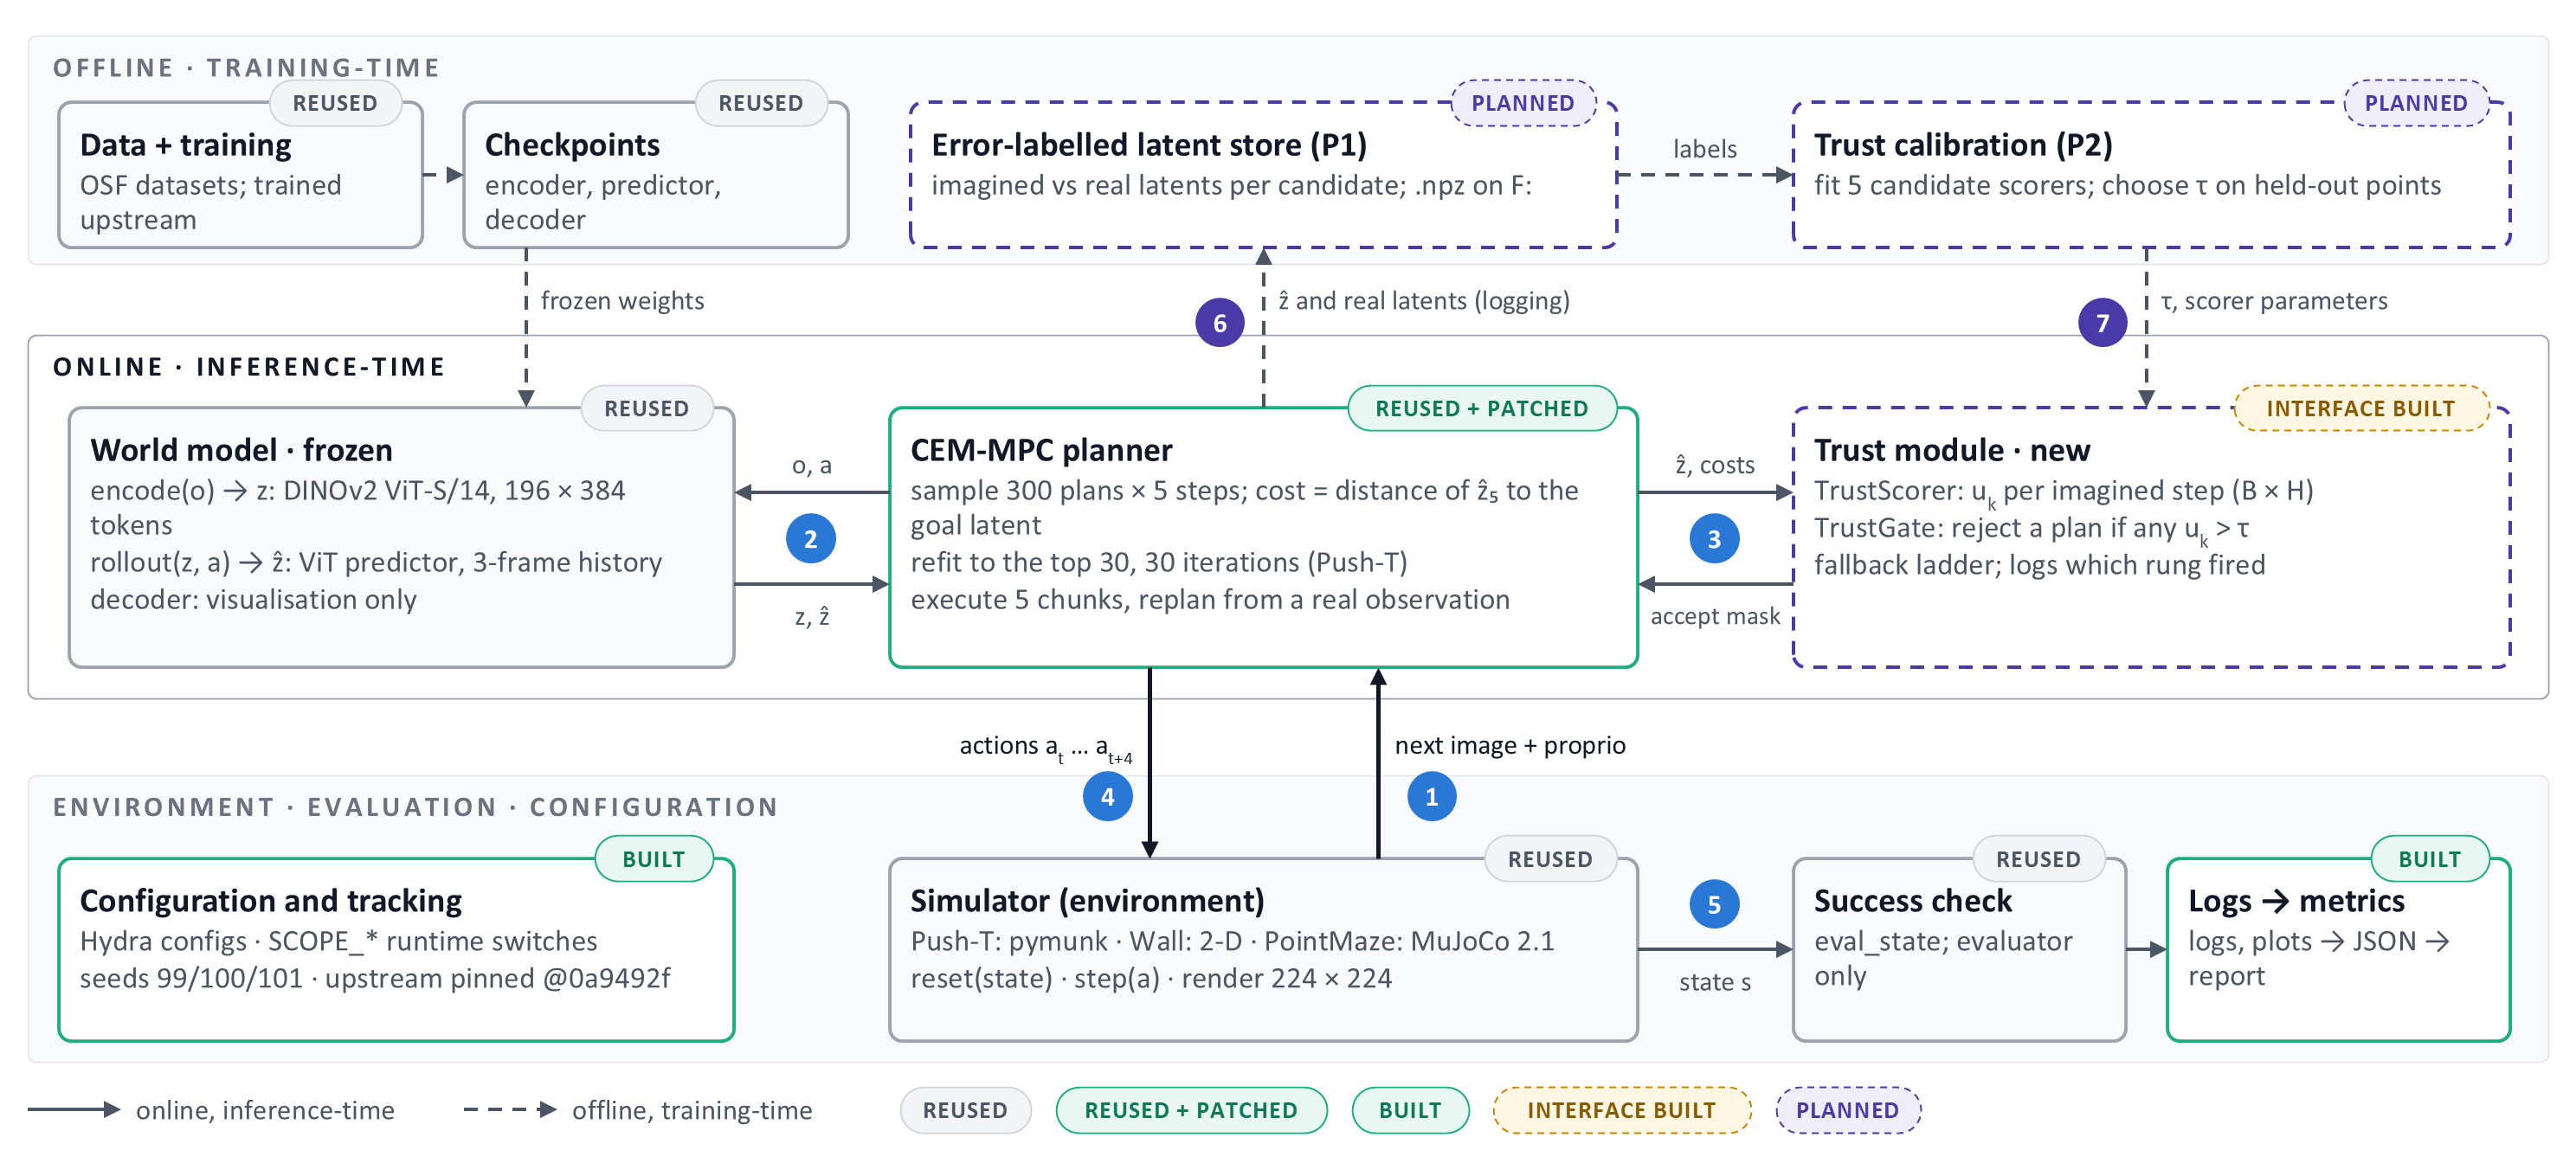
\includegraphics[width=0.92\textwidth]{figures/fig_architecture.png}
\caption{SCoPe system architecture. Middle: the agent at decision time (frozen DINO-WM, CEM-MPC planner and the trust
module). Top: the offline loop that logs imagined against real latents and calibrates the scores. Status tags mark
reused, built, interface-only and planned components.}
\label{fig:arch}
\end{figure*}

\subsection{Architecture}
Fig.~\ref{fig:arch} shows the system. At each decision the simulator returns an observation, the planner asks the world
model to encode it and imagine the candidates, the trust module scores every imagined step, and only accepted candidates
compete on cost. Offline, imagined latents are logged next to the encodings of what really happened; this
error-labelled data calibrates the scores and $\tau$. The world model is never retrained. Backbones and scorers plug in
through two small interfaces, so V-JEPA~2-AC can replace DINO-WM later.

\subsection{Trust scores}
All scores are computed from the imagination alone, need no training, and are larger for less trusted steps:
\begin{itemize}
\item \textbf{MC-dropout}~\cite{ref23}: variance of $\hat z_k$ over four predictor passes with its dropout (0.1, as trained) on.
\item \textbf{Action perturbation}: divergence of the imagined rollout when the actions receive Gaussian noise ($\sigma=0.1$).
\item \textbf{Image perturbation}, in the spirit of~\cite{ref19}: divergence when the start image receives noise ($\sigma=0.1$).
\item \textbf{Distance to training data}: mean distance to the five nearest encoded training frames (random projection to 512 dimensions).
\item \textbf{Imagined cost}: the plan's own predicted distance to the goal.
\item Controls: \textbf{distance moved}, $\lVert\hat z_k-z_0\rVert$, a trivial score, and \textbf{random}.
\end{itemize}

\subsection{Gated CEM-MPC with a fallback ladder}
Algorithm~\ref{alg:scope} gives the decision loop. Imagined latents are never used as the start of the next plan: after
executing the accepted actions, the agent observes again. When too few candidates pass, the ladder widens the search,
then shortens the horizon, then takes a safe no-op, and logs which rung fired.

\begin{algorithm}[t]
\caption{SCoPe decision step (one MPC round)}\label{alg:scope}
\begin{algorithmic}[1]
\State observe $o_t$; $z_t\gets E(o_t)$
\For{CEM iteration $i=1,\dots,I$}
  \State sample $N$ action sequences $a^{(n)}_{1:H}\sim\mathcal{N}(\mu,\Sigma)$
  \State imagine $\hat z^{(n)}_{1:H}$ with $f_\theta$; score $u^{(n)}_k$ for every step
  \State accepted $\mathcal{A}\gets\{n:\max_k u^{(n)}_k\le\tau\}$
  \If{$|\mathcal{A}|<K$} \State fallback: resample wider $\rightarrow$ $H\gets H/2$ $\rightarrow$ no-op (logged) \EndIf
  \State refit $(\mu,\Sigma)$ to the $K$ lowest-cost candidates in $\mathcal{A}$
\EndFor
\State execute the first chunks of the best accepted plan; return to line 1
\end{algorithmic}
\end{algorithm}

\subsection{Hypotheses}
H1: a trust score ranks steps with large real latent error above the others (AUROC, Spearman $\rho$). H2/H3: the gate's
false rejections (plans that would have succeeded) and false acceptances stay below a random gate's. H4: gating raises
real success over plain MPC, a soft uncertainty penalty and a random gate, with an oracle gate (rejecting on the true
error) as the upper bound. Go/no-go: the closed loop is built only if a score beats both the random and the trivial
control on H1 with non-overlapping 95\% intervals.

% ======================================================================
\section{Experimental Setup}

\textbf{Tasks and data.} Push-T~\cite{ref24} (push a T-shaped block onto a target), Wall (pass through a door) and
PointMaze~\cite{ref25}, with the datasets and released checkpoints of DINO-WM~\cite{ref26}. Push-T goals are the real
state 25 steps later on a held-out trajectory; Wall and PointMaze goals are sampled reachable states.

\textbf{Planner.} Upstream settings: 300 samples, top 30, horizon 5, 30 CEM iterations on Push-T and 10 on Wall and
PointMaze, five chunks executed per MPC round, at most three rounds (the paper does not state its replanning budget, so
we report every round). 50 start/goal pairs per seed; seeds 99, 100 and 101. We read the paper's CEM row as our round~1
(one plan, executed open loop) and its MPC row as success after replanning.

\textbf{Hardware and runtime patches.} One RTX~5060 laptop GPU (8\,GB), WSL2, PyTorch~2.7.1 with CUDA~12.8. Unmodified,
a 300-candidate rollout took 26.2\,s and did not fit in memory at full settings. We fused attention, encoded the shared
observation once instead of 300 times, chunked rollouts, disabled autograd where unused, and enabled TF32 matrix
multiplication: 6.9\,s per rollout (3.8$\times$). Against the unmodified model, CEM's top-30 set and its update were
identical at three sampling spreads; bf16 was faster but changed 17\% of the elites at small spreads and was rejected.
(These benchmark figures are from our benchmark script, not from the generated tables.)

\textbf{H1 pilot protocol.} On \HEpisodes{} Push-T decision points over \HSeedWord{}, CEM ran 10 iterations; we recorded
192 of the candidates it evaluated per decision point (48 from iteration~1, 48 from iteration~5 and 96 from
iteration~10, so the set spans bad to good plans), imagined each, executed each from the same start state in the
simulator, and encoded the real frames at steps 5,\,10,\,\dots,\,25: \HPairs{} imagined steps with a real latent next to
them. The real error of step $k$ is the mean squared difference of the imagined and real patch tokens; a step is
\emph{unreliable} if its error is in the top 10\% \emph{for its step index}, so that the growth of error with the horizon
cannot inflate a score. AUROC and Spearman $\rho$ are computed per step and averaged; 95\% intervals come from 500
bootstrap resamples over decision points.

\textbf{Offline gate replay.} Among each decision point's recorded candidates, plain selection takes the lowest imagined
cost; a gate first rejects the 30\% least trusted candidates (by their worst step). The outcome is whether the chosen
candidate succeeds in the simulator. This is a hint for H4, not H4.

% ======================================================================
\section{Results}

\subsection{Reproduction of DINO-WM}

\begin{table}[t]
\caption{Planning success over 50 start/goal pairs per seed (mean $\pm$ SD over seeds).}
\label{tab:phase0}
\centering
\setlength{\tabcolsep}{3pt}
\resizebox{\columnwidth}{!}{\begin{tabular}{@{}lcccc@{}}
\toprule
Task & Seeds & One plan (round 1) & With replanning & Paper~\cite{ref1} \\
\midrule
Push-T & 3 & 0.87 $\pm$ 0.05 & 0.90 $\pm$ 0.05 (round 3) & 0.86 / 0.90 \\
Wall & 3 & 0.52 $\pm$ 0.02 & 0.95 $\pm$ 0.02 (round 3) & 0.74 / 0.96 \\
PointMaze & 1 & 0.86 & 1.00 (round 2) & 0.80 / 0.98 \\
\bottomrule
\end{tabular}
}
\end{table}

Table~\ref{tab:phase0} summarises the reproduction. On Push-T we obtain \PushTRoneMean{}~$\pm$~\PushTRoneSD{} after one
plan and \PushTFinalMean{}~$\pm$~\PushTFinalSD{} after replanning (per seed \PushTPerSeedFinal{}), against the published
0.86 and 0.90; at 50 pairs the binomial standard error is about 0.04, so both published values lie within the seed spread.
PointMaze reaches \MazeFinalMean{} after round \MazeFinalRound{} (published 0.98). Wall reaches \WallFinalMean{} after
round \WallFinalRound{} (per seed \WallPerSeedFinal{}; published 0.96), but its single-plan result,
\WallRoneMean{}~$\pm$~\WallRoneSD{}, is consistently below the published 0.74. We do not know why yet; the upstream Wall
setting stops CEM after 10 iterations, and our mapping of the paper's CEM row to round~1 may not match its protocol.
Fig.~\ref{fig:cem} shows that on Push-T the success of CEM's current plan rises steeply in the first ten iterations and
plateaus after about twenty.

\begin{figure}[t]
\centering
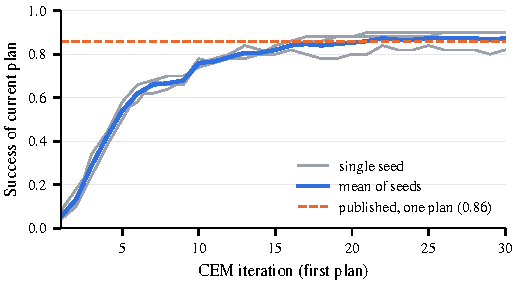
\includegraphics[width=\columnwidth]{figures/fig_cem.pdf}
\caption{Push-T, first plan: success rate of CEM's current mean plan after each iteration (evaluation only; the planner
never sees it). Grey: seeds; blue: mean; dashed: published single-plan result.}
\label{fig:cem}
\end{figure}

\subsection{H1: do trust scores predict real error?}

\begin{table}[t]
\caption{H1 pilot: AUROC for the top-10\% real latent error (per step), \HEpisodes{} Push-T decision points, \HSeedWord{}.}
\label{tab:h1}
\centering
\setlength{\tabcolsep}{4pt}
\resizebox{\columnwidth}{!}{\begin{tabular}{@{}lcc@{}}
\toprule
Trust score & AUROC & 95\% interval \\
\midrule
\textbf{MC-dropout} & \textbf{0.863} & \textbf{0.84--0.88} \\
Action perturbation & 0.657 & 0.64--0.67 \\
Distance to training data & 0.619 & 0.56--0.66 \\
Imagined cost & 0.511 & 0.47--0.55 \\
Image perturbation & 0.496 & 0.44--0.55 \\
\midrule
Distance moved (baseline) & 0.790 & 0.76--0.82 \\
Random (baseline) & 0.500 & 0.49--0.51 \\
\bottomrule
\end{tabular}
}
\end{table}

\begin{figure}[t]
\centering
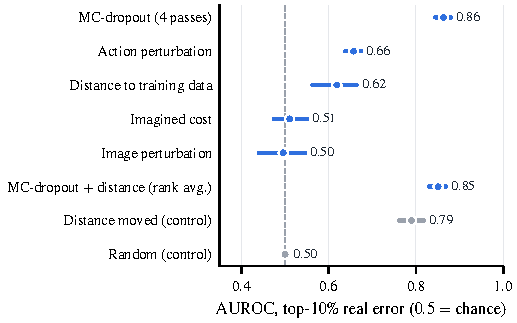
\includegraphics[width=\columnwidth]{figures/fig_auroc.pdf}
\caption{AUROC with 95\% bootstrap intervals over decision points. Blue: candidate trust scores; grey: controls;
dashed: chance.}
\label{fig:auroc}
\end{figure}

Table~\ref{tab:h1} and Fig.~\ref{fig:auroc} answer H1 for this pilot. MC-dropout ranks the unreliable steps highest, with
AUROC \HMC{} (95\% CI \HMCCI{}; per seed \HMCPerSeed{}), and its whole interval lies above the trivial control
(\HDist{}, \HDistCI{}) and the random score (\HRand{}). It is the only score that passes the go/no-go criterion. Action
perturbation (\HAct{}) and distance to the training data (\HKnn{}) carry some signal but less than the trivial control.
The plan's own imagined cost carries none (\HCost{}): a confident planner is no evidence of a correct imagination. Image
perturbation is at chance (\HObs{}), most likely because small noise on the input image is absorbed by the frozen
encoder, so it probes the encoder rather than the predictor. The strength of the trivial control is itself informative:
plans that change the scene a lot are the ones the model gets wrong, so every score must be compared with it, not only
with chance. A rank average of MC-dropout and the trivial control, fixed in advance, does not improve on MC-dropout alone
(Table~\ref{tab:h1}).

\subsection{Offline gate replay}

\begin{table}[t]
\caption{Offline gate replay (reject 30\%, then lowest imagined cost).}
\label{tab:gate}
\centering
\begin{tabular}{@{}lc@{}}
\toprule
Selection among recorded candidates & Chosen plan succeeds \\
\midrule
Plain (lowest imagined cost) & 71.3\% \\
Oracle gate (true error) & 72.5\% \\
Random gate & 70\% \\
MC-dropout gate & 70\% \\
Action-perturbation gate & 75\% \\
Distance-to-data gate & 68.8\% \\
Distance-moved gate & 67.5\% \\
\bottomrule
\end{tabular}

\end{table}

Table~\ref{tab:gate} shows the replay. The plan chosen without a gate succeeds in \GatePlain{} of decision points, and
\GateMC{} with the MC-dropout gate; one decision point is worth \GateStep{}, so the differences between gates are within
noise. The informative row is the oracle: even rejecting by the \emph{true} error barely changes success (\GateOracle{} against \GatePlain{}). Among the
recorded candidates, the one with the lowest imagined cost is rarely a high-error one, so a one-shot gate has little to
change. Predicting error (H1) is therefore necessary but not sufficient; whether rejection changes what the agent does
over several replanning rounds, and in harder conditions, is the question for H4.

% ======================================================================
\section{Discussion and Limitations}

The evidence for SCoPe so far is offline and from one task: three seeds and \HEpisodes{} decision points, one sampling
context (CEM's first plan), no calibration error yet, and no closed-loop result. The pilot shows that the logging pipeline
works and that a cheap, untrained score tracks real error well beyond a strong trivial baseline; it does not show that
gating helps, and the oracle replay suggests the gain, if any, will come from changing decisions across rounds and from
harder or shifted conditions rather than from filtering the final candidates. All tasks are simulated and 2-D; real-world
validity would require a backbone such as V-JEPA~2-AC with robot data. Planning takes minutes per decision on our GPU,
so the system is not real-time. Upstream MPC stops solved episodes using the simulator's success flag; we keep this
identical for every method.

% ======================================================================
\section{Conclusion and Future Work}

We reproduced DINO-WM planning on an 8\,GB GPU within the published results on Push-T, PointMaze and, after replanning,
Wall, with a 3.8$\times$ faster runtime that leaves the planner's choices unchanged. A first test of SCoPe's central
hypothesis found that an untrained MC-dropout score identifies the most wrong imagined steps (AUROC \HMC{}), clearly
above random and above a strong trivial control, while an offline gate replay showed almost no change in success, even for an
oracle. Next steps: more decision points, the remaining sampling contexts (dataset states, perturbed starts and
visual shifts that leave the dynamics unchanged), calibration, an ensemble score, and then the closed-loop gate with its
fallback ladder against plain MPC, a soft penalty, a random gate and the oracle gate on Push-T, Wall and PointMaze.

\section*{Reproducibility}
Code, run scripts and the report sources are in the project repositories (scope-planning, scope-project,
scope-mid-review). Every number in Tables~\ref{tab:phase0}--\ref{tab:gate} and in the text is generated from the run logs
by \texttt{report/make\_assets.py}.

\balance
% generated by report/make_bib.js from docs/mid_review/src/refs.js; do not edit
\begin{thebibliography}{99}
\small
\bibitem{ref1} G. Zhou, H. Pan, Y. LeCun, L. Pinto. DINO-WM: World Models on Pre-trained Visual Features enable Zero-shot Planning. ICML 2025, PMLR 267:79115--79135. \url{https://arxiv.org/abs/2411.04983}

\bibitem{ref2} M. Assran et al. V-JEPA 2: Self-Supervised Video Models Enable Understanding, Prediction and Planning. arXiv:2506.09985, 2025. \url{https://arxiv.org/abs/2506.09985}

\bibitem{ref3} M. Oquab et al. DINOv2: Learning Robust Visual Features without Supervision. TMLR, 2024. \url{https://arxiv.org/abs/2304.07193}

\bibitem{ref4} M. Assran et al. Self-Supervised Learning from Images with a Joint-Embedding Predictive Architecture (I-JEPA). ICCV 2023. \url{https://arxiv.org/abs/2301.08243}

\bibitem{ref5} Y. LeCun. A Path Towards Autonomous Machine Intelligence. Position paper, v0.9.2, 2022 (not peer-reviewed). \url{https://openreview.net/forum?id=BZ5a1r-kVsf}

\bibitem{ref6} K. Chua, R. Calandra, R. McAllister, S. Levine. Deep Reinforcement Learning in a Handful of Trials using Probabilistic Dynamics Models (PETS). NeurIPS 2018. \url{https://arxiv.org/abs/1805.12114}

\bibitem{ref7} D. Hafner et al. Learning Latent Dynamics for Planning from Pixels (PlaNet). ICML 2019, PMLR 97:2555--2565. \url{https://arxiv.org/abs/1811.04551}

\bibitem{ref8} M. Janner, J. Fu, M. Zhang, S. Levine. When to Trust Your Model: Model-Based Policy Optimization (MBPO). NeurIPS 2019. \url{https://arxiv.org/abs/1906.08253}

\bibitem{ref9} T. Yu et al. MOPO: Model-based Offline Policy Optimization. NeurIPS 2020. \url{https://arxiv.org/abs/2005.13239}

\bibitem{ref10} R. Kidambi, A. Rajeswaran, P. Netrapalli, T. Joachims. MOReL: Model-Based Offline Reinforcement Learning. NeurIPS 2020. \url{https://arxiv.org/abs/2005.05951}

\bibitem{ref11} B. Frauenknecht, A. Eisele, D. Subhasish, F. Solowjow, S. Trimpe. Trust the Model Where It Trusts Itself: Model-Based Actor-Critic with Uncertainty-Aware Rollout Adaption (MACURA). arXiv:2405.19014, 2024. \url{https://arxiv.org/abs/2405.19014}

\bibitem{ref12} D. Hafner, J. Pasukonis, J. Ba, T. Lillicrap. Mastering Diverse Control Tasks through World Models (DreamerV3). Nature 640:647--653, 2025. \url{https://doi.org/10.1038/s41586-025-08744-2}

\bibitem{ref13} N. Hansen, H. Su, X. Wang. TD-MPC2: Scalable, Robust World Models for Continuous Control. ICLR 2024. \url{https://arxiv.org/abs/2310.16828}

\bibitem{ref14} V. Sobal et al. Learning from Reward-Free Offline Data: A Case for Planning with Latent Dynamics Models (PLDM). NeurIPS 2025. \url{https://arxiv.org/abs/2502.14819}

\bibitem{ref15} W. Zhang et al. Hierarchical Planning with Latent World Models (HWM). arXiv:2604.03208, 2026. \url{https://arxiv.org/abs/2604.03208}

\bibitem{ref16} J. Seo, K. Nakamura, A. Bajcsy. Uncertainty-aware Latent Safety Filters for Avoiding Out-of-Distribution Failures. CoRL 2025. \url{https://arxiv.org/abs/2505.00779}

\bibitem{ref17} J. Berger, B. Frauenknecht, S. Trimpe, B. Leibe. Biased Dreams: Limitations to Epistemic Uncertainty Quantification in Latent Dynamics Models. RLC 2026. \url{https://arxiv.org/abs/2604.25416}

\bibitem{ref18} Z. Wang. Learning from World Feedback: Why Model Uncertainty Fails as a Risk Signal in Model-Based RL. ICML 2026 Workshop on RL from X Feedback. \url{https://arxiv.org/abs/2607.16591}

\bibitem{ref19} G. An et al. Diagnosing JEPA World Models with Action-Conditioned Predictive Consistency (ACPC). arXiv:2608.12939, 2026. \url{https://arxiv.org/abs/2608.12939}

\bibitem{ref20} J. Hu et al. Representation Geometry Matters for Planning with JEPA World Models. arXiv:2608.16287, 2026 (arXiv title spells "Reperesentation"). \url{https://arxiv.org/abs/2608.16287}

\bibitem{ref21} G. Lee, B.-T. Zhang. Beyond Task Success: Stage-Wise Reliability of World Model Planning under Sensing Degradation. arXiv:2609.07126, 2026. \url{https://arxiv.org/abs/2609.07126}

\bibitem{ref22} B. Lakshminarayanan, A. Pritzel, C. Blundell. Simple and Scalable Predictive Uncertainty Estimation using Deep Ensembles. NIPS 2017. \url{https://arxiv.org/abs/1612.01474}

\bibitem{ref23} Y. Gal, Z. Ghahramani. Dropout as a Bayesian Approximation: Representing Model Uncertainty in Deep Learning. ICML 2016. \url{https://arxiv.org/abs/1506.02142}

\bibitem{ref24} C. Chi et al. Diffusion Policy: Visuomotor Policy Learning via Action Diffusion. RSS 2023 (origin of the Push-T task used by DINO-WM). \url{https://arxiv.org/abs/2303.04137}

\bibitem{ref25} J. Fu, A. Kumar, O. Nachum, G. Tucker, S. Levine. D4RL: Datasets for Deep Data-Driven Reinforcement Learning. arXiv:2004.07219, 2020 (PointMaze). \url{https://arxiv.org/abs/2004.07219}

\bibitem{ref26} DINO-WM code (MIT licence), pinned at commit 0a9492f; datasets and checkpoints on OSF (project bmw48). \url{https://github.com/gaoyuezhou/dino_wm}
\end{thebibliography}


\end{document}
